%%% LaTeX Template: Two column article
%%%
%%% Source: http://www.howtotex.com/
%%% Feel free to distribute this template, but please keep to referal to http://www.howtotex.com/ here.
%%% Date: February 2011

%%% Preamble
\documentclass[	DIV=calc,%
							paper=a4,%
							fontsize=12pt,%
							onecolumn]{scrartcl}	 					% KOMA-article class

\usepackage{lipsum}													% Package to create dummy text
\usepackage[brazil]{babel}										% English language/hyphenation
\usepackage[protrusion=true,expansion=true]{microtype}				% Better typography
\usepackage{amsmath,amsfonts,amsthm}					% Math packages
\usepackage[pdftex]{graphicx}									% Enable pdflatex
\usepackage[svgnames]{xcolor}									% Enabling colors by their 'svgnames'
\usepackage[hang, small,labelfont=bf,up,textfont=it,up]{caption}	% Custom captions under/above floats
\usepackage{epstopdf}												% Converts .eps to .pdf
\usepackage{subfig}													% Subfigures
\usepackage{booktabs}												% Nicer tables
\usepackage{fix-cm}													% Custom fontsizes
\usepackage[utf8]{inputenc}
\usepackage[top=2.5cm, bottom=2.5cm, left=2.5cm, right=2.5cm]{geometry}
\usepackage[ddmmyyyy]{datetime}
\addto\captionsenglish{%
	\renewcommand\tablename{Tabela}
	\renewcommand\figurename{Figura}
} 
 

 
%%% Custom sectioning (sectsty package)
\usepackage{sectsty}													% Custom sectioning (see below)
\allsectionsfont{%															% Change font of al section commands
	\usefont{OT1}{phv}{b}{n}%										% bch-b-n: CharterBT-Bold font
	}

\sectionfont{%																% Change font of \section command
	\usefont{OT1}{phv}{b}{n}%										% bch-b-n: CharterBT-Bold font
	}



%%% Headers and footers
\usepackage{fancyhdr}												% Needed to define custom headers/footers
	\pagestyle{fancy}														% Enabling the custom headers/footers
\usepackage{lastpage}	

% Header (empty)
\lhead{}
\chead{}
\rhead{}
% Footer (you may change this to your own needs)

%% ====================================
%% ====================================
%% mude o rodape  do projeto
%% ====================================
%% ====================================

\lfoot{\footnotesize \texttt{Template para entrega de texto} \textbullet ~Modelo de projeto}


\cfoot{}
\rfoot{\footnotesize página \thepage\ de \pageref{LastPage}}	% "Page 1 of 2"
\renewcommand{\headrulewidth}{0.0pt}
\renewcommand{\footrulewidth}{0.4pt}



%%% Creating an initial of the very first character of the content
\usepackage{lettrine}
\newcommand{\initial}[1]{%
     \lettrine[lines=3,lhang=0.3,nindent=0em]{
     				\color{DarkGoldenrod}
     				{\textsf{#1}}}{}}



%%% Title, author and date metadata
\usepackage{titling}															% For custom titles

\newcommand{\HorRule}{\color{DarkGoldenrod}%			% Creating a horizontal rule
									  	\rule{\linewidth}{1pt}%
										}

\pretitle{\vspace{-30pt} \begin{flushleft} \HorRule 
				\fontsize{50}{50} \usefont{OT1}{phv}{b}{n} \color{DarkRed} \selectfont 
				}

\title{Processo de produção de sofware pra saúde}		% Title of your article goes here

%% ====================================



\posttitle{\par\end{flushleft}\vskip 0.5em}

\preauthor{\begin{flushleft}
					\large \lineskip 0.5em \usefont{OT1}{phv}{b}{sl} \color{DarkRed}}
\author{Eduardo Amaral Pereira }  	% Author name goes here


\postauthor{\footnotesize \usefont{OT1}{phv}{m}{sl} \color{Black} 
					\\Universidade Tecnológica Federal do Paraná - Câmpus Cornélio Procópio 								% Institution of author
					\par\end{flushleft}\HorRule}

\date{}																				% No date


%%% Begin document
\begin{document}
\maketitle
\thispagestyle{fancy} 	
\thispagestyle{empty}		% Enabling the custom headers/footers for the first page 
% The first character should be within \initial{}


\initial{E}\textbf{ste documento visa a demonstrar o modelo de produção de software em uma empresa de grande porte(cerca de 200 funcionários). O modelo adotado apresenta o processo de desenvolvimento por meio de editais.}

%% ====================================
\begin{figure}
	\centering
	
\includegraphics{utfpr}
\end{figure}

\vspace{3cm}
\centerline{\textit{\textbf{\today}}}

\clearpage
    \renewcommand*\listfigurename{Lista de figuras}
\listoffigures

\renewcommand*\listtablename{Lista de tabelas}
\listoftables


\clearpage
\renewcommand{\contentsname}{Sumário}
\tableofcontents
\clearpage

%% ====================================
%% ====================================
%% Inicio do texto
%% ====================================
%% ====================================
\section{Introdução}
Este processo é utilizado para a produção de softwares na área da saúde em diversos produtos disponibilizados para
a Auto gestão de saúde e também para Medicina de grupo. Seu foco principal é a implementação de funcionalidades demandadas
de um licitação a qual possui um edital de requisitos a serem cumpridos.

Apenas grupos de Auto Gestão demandam por meio de editais, pois este é o meio utilizado para o gerenciamento da saúde
em orgãos públicos. O segmento de medicina de grupo é voltado para a comercialização de planos de saúde e não se enquadram
aos orgãos públcos para o gerenciamento de vidas.

:

\begin{itemize}
	\item Sistemas de gestão de saúde de Auto Gestão;
	\item Diversos colaboradores, os mesmo serão representados por seus papéis no processo de desenvolvimento;
	\item https://github.com/eamaralp/ProcessoDeSoftware;
\end{itemize}


\section{Processo}
Descreva aqui o processo utilizado.

\subsection{Papeis}
\begin{itemize}
	\item \textbf{Cliente:} Representante do orgão público responsável em auditar o produto a ser desenvolvido.
	\item \textbf{Analista de negócios:} Responsável em realizar a análise de negócio dos editais e realizar a extração dos requisitos contidos nestes. 
	\item \textbf{Gerente de desenvolvimento:} Responsável em gerenciar uma ou mais equipe de desenvolvimento. Deve priorizar,organizar e gerenciar 
	os times de desenvolvimento para garantir que as funcionalidades sejam entregues dentro do cronograma estabelecido.
	\item \textbf{Desenvolvedor:} Responsável em realizar a análise de sistemas, verificando necessidades técnicas e implementar as funcionalidades analisadas.
	\item \textbf{Revisor de código:} Desenvolver com mais conhecimento técnico que exerce o papél de desenvolvedor e também realiza 
	a revisão de código de outros desenvolvedores.
	\item \textbf{Atualizador:} Responsável em aplicar os artefatos gerados durante o desenvolvimento no ambiente de qualidade.
	\item \textbf{Analista de testes:} Responsável em realizar testes nas funcionaliades de acrodo com as análises e verificar se estas não possuem nenhum erro.
\end{itemize}

\subsection{Atividades}

O processo de desenvolvimento de incia no momento em que a empresa é contemplada pela licitação, desta forma uma análise prévia é realizada pelos arquitetos
de negócio com o intuito de verificar requisitos os quais já são contemplados pelos produtos da empresa, desta forma elminando parte deste requisitos e tornando o
custo de implementação das funcionalidades menor. O analista valida os requisitos junto ao cliente, com a intenção de descreve-los da melhor forma porssível e verifica
se este requisitos será implementado em um sistema já existente ou se será necessário desenvlver um novo sistema para que as novas funcionalidades sejam implementadas.

Após a definição dos requisitos os documentos de análise são encaminhados ao gerente de desenvolvimento, o qual define um cronograma de acrodo com as funcionalidades e
sua complexidades, um analista de sistemas esperiente realiza uma estimativa de tempo de implementação de cada funcionalidade para que o gerente de desenvolvimento possa
apresentar um cronograma mais assertivo.

Ao entrar em acordo com o cliente junto ao cronograma o gerente de desenvolvimento encaminha as atividades para as devidas equipes de acordo com a área de atução das mesmas
e o sistema em que serão implementadas. Desta forma o desenvolvimento pode ser realizado de maneira paralela, de acordo com as dependências entre as funcionalidades e sistemas.

Após as funcionalidades serem encaminhadas para a equipe de desenvolvimento, as mesmas são priorizadas e reestimadas pela equipe para que o gestor posssa ter um melhor
detalhamento do cronograma. Após receber sua atividade o desenvolvedor escreve uma breve análise de sistemas, de acrodo com o MODELO() e encaminha para o analista de sistemas
realizar a revisão de sua análise. Depois de aprovada a análise o desenvolvedor incia o desenvolvimento da funcionalidade e ao seu término encaminha o código gerado para
a revisão, a qual será realizada por outro desenvolvedor de maior experiência.


\section{Execução do projeto}

Relacione as atividades com os integrantes, crie um cronograma conforme orientações
\subsection{Backlog e sprints}
-- item obrigatório --

Evidencie todos os stakeholders envolvidos


\subsection{Estado atual}
Apresente os artefatos gerados em ordem cronológica, conforme processo.


\section{Referências bibliográficas}
Utilize o mendley, o jabref ou diretamente o bibtex para gerenciar suas referências biliográficas. As referências são criadas automaticamente de acordo com o uso no texto.

Exemplo: Redes de computadores, segundo \cite{t2013} é considerada..... Já \cite{kurose2010} apresenta uma versão...

Analisando os pressupostos de \cite{ref3} e \cite{ref4} concluimos que....


\renewcommand\refname{} %%Referências bibliográficas}  
\bibliographystyle{ieeetr}
\bibliography{referencias}  

%% ***********************************************************************
%% === remover daqui =====================================================
%% ***********************************************************************
=================================================
\section{Elementos textuais - Alguns exemplos}

Esta seção apresenta exemplos de elementos textuais. \textbf{Remova-a da versão final do texto}.


\subsection{Colocar elementos em itens}

Texto antes da lista

\begin{itemize}
	\item First item in a list 
	\item Second item in a list 
\item Third item in a list
\end{itemize}
\label{}
\subsubsection{Uma subseção de terceiro nivel}

Exemplo de uma subseção

\subsection{Tabelas}

Utilize o site http://www.tablesgenerator.com/ para elaborar as tabelas de seu trabalho.
Para adicionar uma tabela utilize: a tag input, passando o arquivo da tabela como parametro

\label{tab_visao_estatica} 
\begin{table}[]
\begin{tabular}{|l|l|l|l|l|l|l|l|}
\hline
\textbf{Fase} & \textbf{Atividade} & \textbf{Tarefa} & \textbf{Artefato de entrada} & \textbf{Artefato de saída} & \textbf{Habilidades} & \textbf{Papel responsável} & \textbf{Ferramentas} \\ \hline
 &  &  &  &  &  &  &  \\ \hline
 &  &  &  &  &  &  &  \\ \hline
 &  &  &  &  &  &  &  \\ \hline
\end{tabular}
\end{table}

Dentro do arquivo você deve definir o label e pode utilizá-lo para referenciar. Exemplo:
Na tab \ref{tab_visao_estatica} temos a relação de ....


Você também pode modificar a tabela manualmente, incluindo, por exemplo h! dentro de sua definição. Veja no exemplo tab2.tex

\subsection{Figuras}

Não se preocupe o local em que a figura será renderizada em seu texto. Preocupe-se em criar referência para ela, ou seja, toda figura e tabela deve conter pelo menos uma referência no texto.

\begin{figure}
\centering
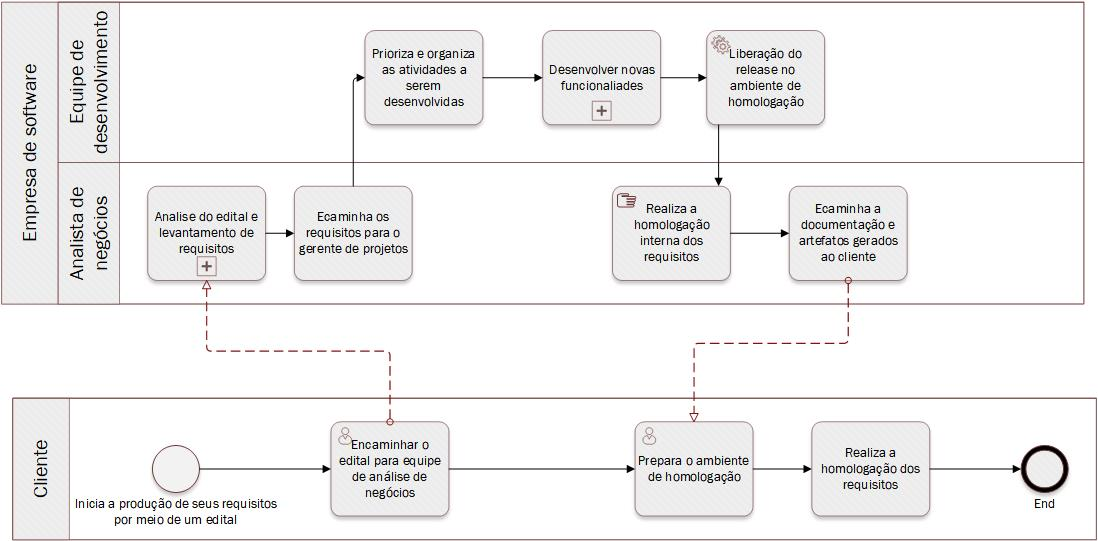
\includegraphics[width=\textwidth]{processo_de_software_BPMN1}
\caption{Exemplo de figura com escala horizontal}
\end{figure}


\begin{figure}
	\centering
	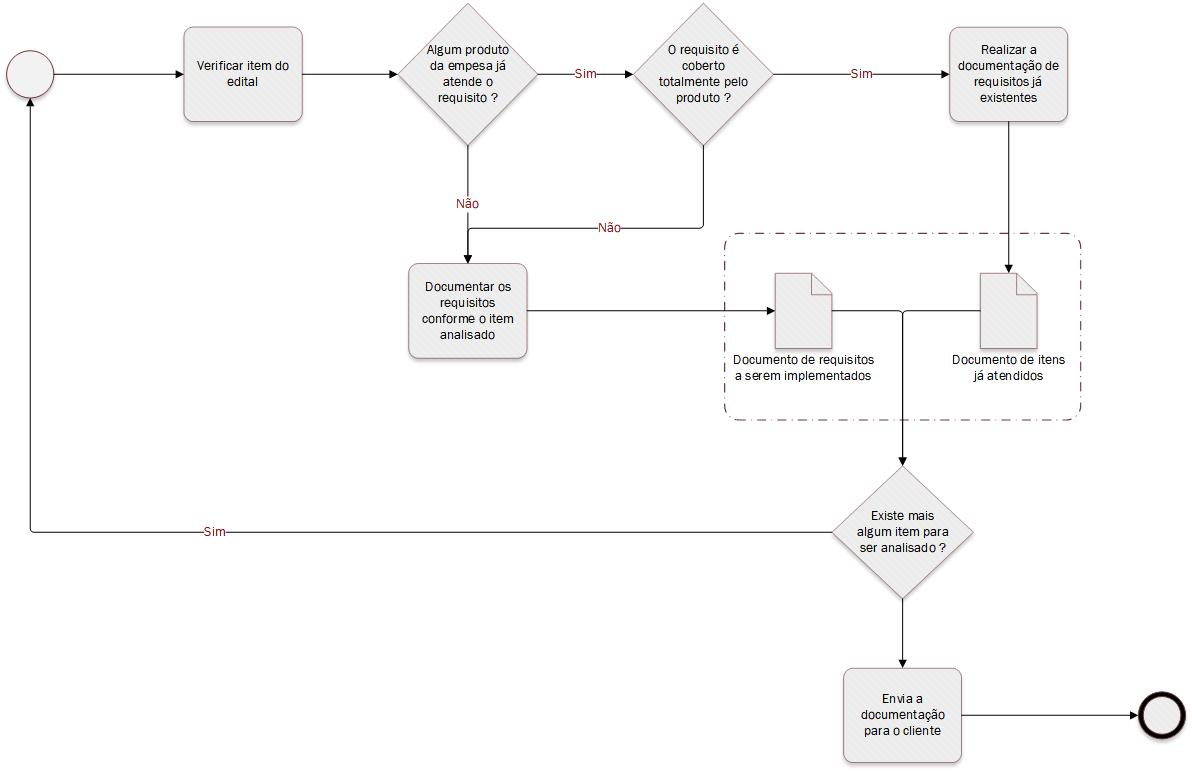
\includegraphics[width=\textwidth]{processo_de_software_BPMN2}
	\caption{Exemplo de figura sem escala}
	\label{fig2}
\end{figure}

\begin{figure}
	\centering
	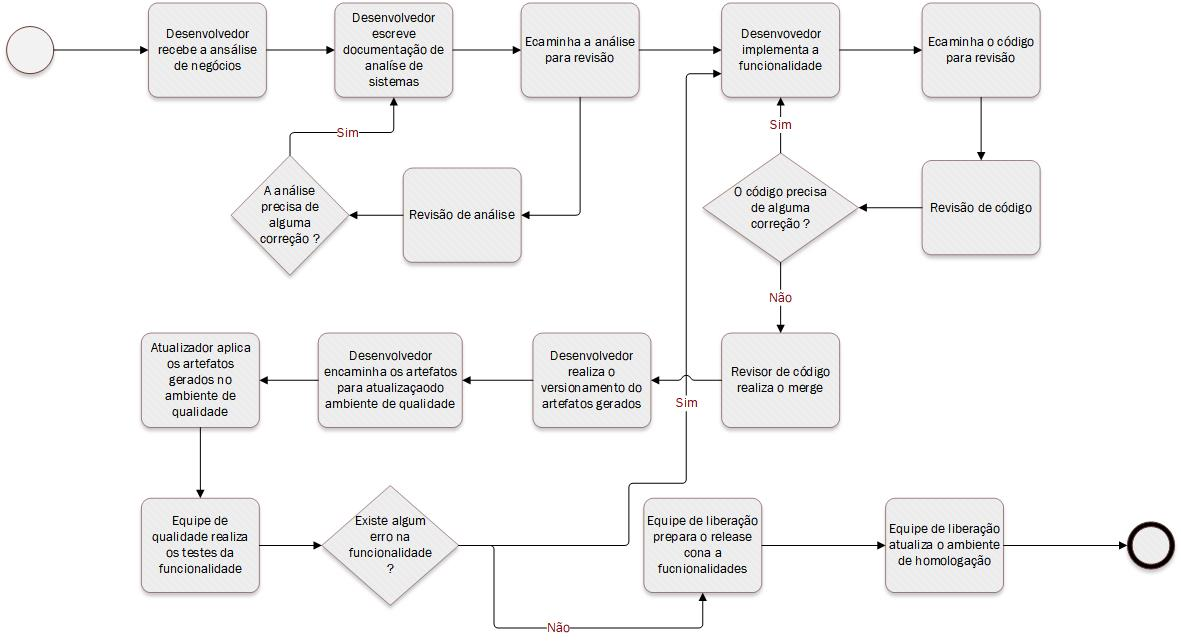
\includegraphics[width=\textwidth]{processo_de_software_BPMN3}
	\caption{Exemplo de figura sem escala}
	\label{fig2}
\end{figure}

%% ***********************************************************************
%% === ate aqui    =====  ================================================
%% ***********************************************************************

\end{document}